\section{Evidence for each stage of the final pipeline}
\label{sec:supp_stages}
Figure~\ref{fig:supp_stages_full} repeats Fig.~2 of the main paper with every intermediate map.

\begin{figure*}[t]
\centering
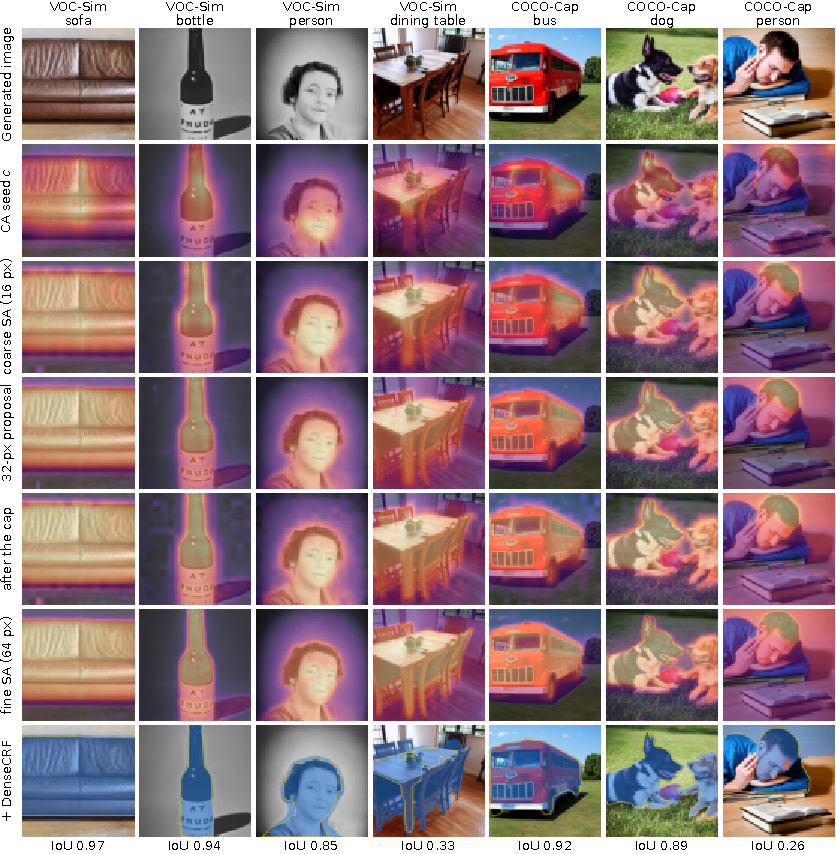
\includegraphics[width=.9\textwidth]{figures/supp_pipeline_c2f.pdf}
\caption{\textbf{Every stage, same fixed-rule images as Fig.~2 of the main paper.} Rows: generated image; A3 seed; coarse 16-pixel SA $r$; 32-pixel proposal $q$; capped map $z$; fine 64-pixel SA $y$; final mask after DenseCRF with the annotation outline. Regenerated maps reproduce the committed per-image scores (largest image-IoU difference 0.005, one COCO-Cap image).}
\label{fig:supp_stages_full}
\end{figure*}

\subsection{Seed}
Figure~\ref{fig:supp_seeds} shows the per-resolution CA maps. 8-pixel CA is blob-like and 16-pixel CA follows object parts, while 64-pixel CA fires on texture and edges throughout the image. A3 down-weights the 64-pixel modules, so its seed is smoother than the uniform one. Table~\ref{tab:supp_sg24} lists every weighting scheme of the same run. Per-pixel content-token rescaling (A1, A4) collapses on COCO-Cap, where the attribution prompt has a single content token, and projected-output head weighting (A2) loses on both benchmarks.

\begin{figure*}[t]
\centering
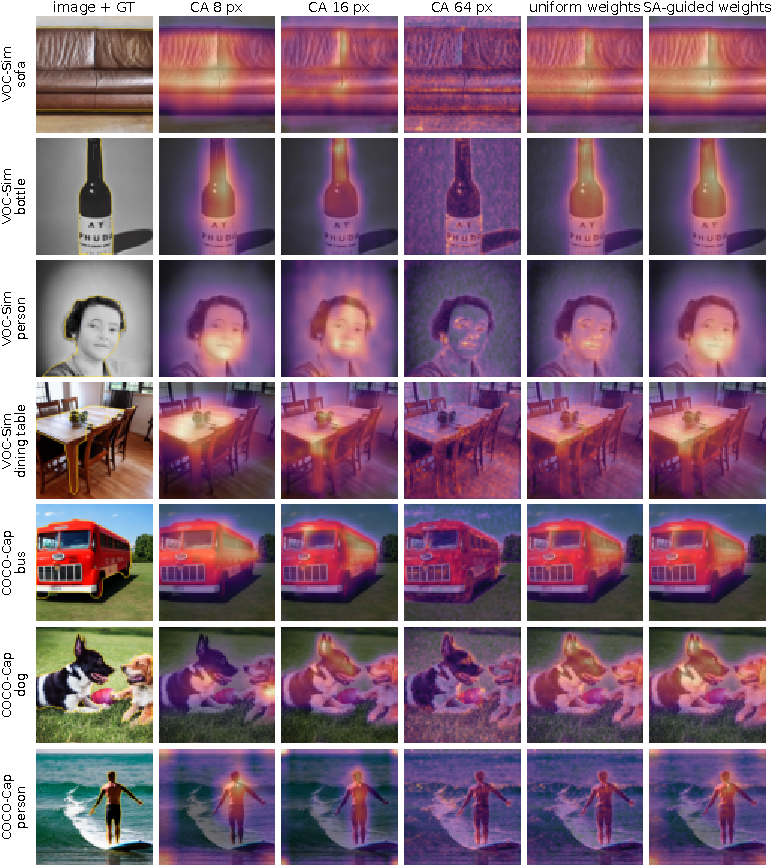
\includegraphics[width=.8\textwidth]{figures/supp_ca_seeds.pdf}
\caption{\textbf{CA by resolution.} Unweighted mean CA of the selected modules at 8, 16 and 64 pixels, the uniform seed and the A3 seed, for the images of Fig.~2 of the main paper.}
\label{fig:supp_seeds}
\end{figure*}

\begin{table}[t]
\centering
\footnotesize\setlength{\tabcolsep}{3pt}
\begin{tabular}{@{}lccc@{}}
\toprule
Weighting & CA only & final (MID-P2+R2) & COCO final \\
\midrule
A0 uniform & .7135 & .8169 & .6437 \\
A1 content-token mass & .6406 & .8005 & .0000 \\
A2 projected head output & .6897 & .8033 & .6366 \\
A3 SA agreement & .7049 & \textbf{.8230} & \textbf{.6620} \\
A4 all three & .6288 & .8004 & .0000 \\
\bottomrule
\end{tabular}
\caption{\textbf{CA weighting schemes} (one run, VOC forced OOF, COCO-Cap frozen). A3 won 4/5 folds against A0 (paired mean-image interval positive). The registered multi-candidate screen chose A3 in only 3/5 folds and kept A0. A3 was adopted afterwards by owner decision.}
\label{tab:supp_sg24}
\end{table}

\subsection{Coarse and fine SA}
Table~\ref{tab:supp_sg25} gives every scale cell of the run behind Fig.~3 of the main paper. Coarse 16-pixel SA alone is far below fine SA on VOC-Sim but competitive on COCO-Cap after R2 (0.665 vs.\ 0.662). Going from 16 to 64 pixels gains on COCO-Cap but not on VOC-Sim, the gap that the cap closes. The reverse order (64$\rightarrow$16) fails, so the order of the scales matters.

\begin{table}[t]
\centering
\footnotesize\setlength{\tabcolsep}{3pt}
\begin{tabular}{@{}lcccc@{}}
\toprule
Propagation (two passes) & VOC & VOC + R2 & COCO & COCO + R2 \\
\midrule
64 px only (fine) & .8097 & .8228 & .6599 & .6621 \\
16 px only (coarse) & .7225 & .7538 & .6282 & .6652 \\
32 px only & .7924 & .8138 & .6693 & .6948 \\
16 $\rightarrow$ 64 & .8020 & .8170 & .6869 & .6975 \\
32 $\rightarrow$ 64 & .8089 & .8217 & .6695 & .6717 \\
64 $\rightarrow$ 16 & .7505 & .7825 & .6403 & .6705 \\
\bottomrule
\end{tabular}
\caption{\textbf{SA scale and order} (one run, A3 seed, calls 10--20; VOC forced OOF, COCO-Cap frozen).}
\label{tab:supp_sg25}
\end{table}

\subsection{The hierarchy: every variant}
Table~\ref{tab:supp_hier} adds the cells omitted from Table~3 of the main paper: budgeted completion (v1 C7--C9), gated completion (v2 V6), and three single changes to the capped hierarchy. The three changes are a cap applied to each head before averaging (W1), a native 16-pixel seed instead of the downsampled one (W2), and a temporal cap of each call by the running mean of earlier calls (W3). None improves on the one-sided cap. The cap binds in 58\% (VOC-Sim) and 65\% (COCO-Cap) of $2\times2$ groups but removes only 7.6\% and 8.3\% of the proposal mass (mean scaling factor of binding groups 0.84).

\begin{table*}[t]
\centering
\footnotesize\setlength{\tabcolsep}{4pt}
\begin{tabular}{@{}llccc@{}}
\toprule
Run & Variant & VOC raw & VOC + R2 & COCO + R2 \\
\midrule
v1 & relaxed conservation, halfway to the projection at both transitions (C5) & .7926 & .8149 & .7059 \\
v1 & exact conservation (both) + background-only completion budget (C7) & .7785 & .8047 & .7054 \\
v1 & exact conservation (both) + semantic/background odds budget (C8) & .7774 & .8031 & .7061 \\
v1 & relaxed conservation + odds budget (C9) & .7951 & .8140 & .7057 \\
v2 & one-sided cap + completion only where $P_1\ge B$ (V6) & .8143 & .8256 & .6792 \\
\midrule
v3 & one-sided cap, reference (R1, = v2 V3) & .8157 & .8293 & .6964 \\
v3 & head-wise cap: $z=\frac18\sum_h\operatorname{cap}(r,A^{32}_hUr)$ (W1) & .8161 & .8294 & .6972 \\
v3 & native 16-px CA seed $c^\ast_{16}$ instead of $D(c)$ (W2) & .8155 & .8281 & .6975 \\
v3 & temporal cap by the mean of earlier calls (W3) & .8116 & .8261 & .6828 \\
\bottomrule
\end{tabular}
\caption{\textbf{Remaining hierarchy variants} (VOC forced OOF, COCO-Cap frozen; each run has its own same-generation references, which agree with Table~3 of the main paper to 0.0003). Against R1 after R2: W1 $+0.0001$ (CI spans 0), W2 $-0.0012$ (2/5), W3 $-0.0032$ (1/5). The head-wise cap removes almost the same mass (7.7\% vs.\ 7.6\%). The native seed correlates 0.996 with $D(c)$. The temporal cap hurts most on small objects ($-0.016$ in the smallest GT-area bin).}
\label{tab:supp_hier}
\end{table*}


\subsection{DenseCRF}
Across the 490 VOC-Sim images, DenseCRF changes the capped pipeline's image IoU by more than 0.005 in 375 images, improving 278. On COCO-Cap it improves 427 of 707 images and 18 of 20 classes (Table~4 of the main paper). Figure~\ref{fig:supp_crf_classes} shows the per-class change.

\begin{figure}[t]
\centering
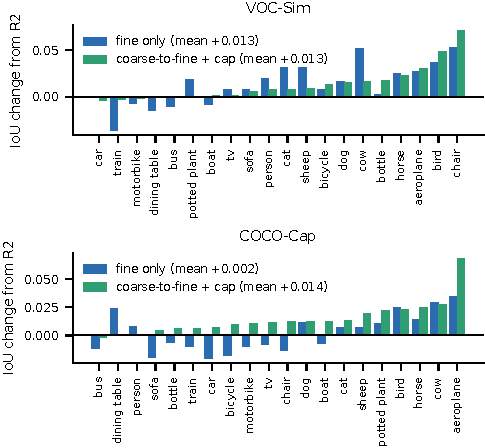
\includegraphics[width=\columnwidth]{figures/supp_crf_classes.pdf}
\caption{\textbf{Per-class effect of DenseCRF} on fine-only and capped coarse-to-fine maps (same run; thresholds from VOC-Sim).}
\label{fig:supp_crf_classes}
\end{figure}
\clearpage
